\documentclass{ximera}

%\usepackage{todonotes}

\newcommand{\todo}{}

\usepackage{esint} % for \oiint
\graphicspath{
{./}
{functionsOfSeveralVariables/}
{normalVectors/}
{lagrangeMultipliers/}
{vectorFields/}
{greensTheorem/}
{shapeOfThingsToCome/}
}


\usepackage{tkz-euclide}
\tikzset{>=stealth} %% cool arrow head
\tikzset{shorten <>/.style={ shorten >=#1, shorten <=#1 } } %% allows shorter vectors

\usetikzlibrary{backgrounds} %% for boxes around graphs
\usetikzlibrary{shapes,positioning}  %% Clouds and stars
\usetikzlibrary{matrix} %% for matrix
\usepgfplotslibrary{polar} %% for polar plots
\usetkzobj{all}
\usepackage[makeroom]{cancel} %% for strike outs
%\usepackage{mathtools} %% for pretty underbrace % Breaks Ximera
\usepackage{multicol}
\usepackage{pgffor} %% required for integral for loops


%% http://tex.stackexchange.com/questions/66490/drawing-a-tikz-arc-specifying-the-center
%% Draws beach ball
\tikzset{pics/carc/.style args={#1:#2:#3}{code={\draw[pic actions] (#1:#3) arc(#1:#2:#3);}}}



\usepackage{array}
\setlength{\extrarowheight}{+.1cm}   
\newdimen\digitwidth
\settowidth\digitwidth{9}
\def\divrule#1#2{
\noalign{\moveright#1\digitwidth
\vbox{\hrule width#2\digitwidth}}}





\newcommand{\RR}{\mathbb R}
\newcommand{\R}{\mathbb R}
\newcommand{\N}{\mathbb N}
\newcommand{\Z}{\mathbb Z}

%\newcommand{\sage}{\textsf{SageMath}}


%\renewcommand{\d}{\,d\!}
\renewcommand{\d}{\mathop{}\!d}
\newcommand{\dd}[2][]{\frac{\d #1}{\d #2}}
\newcommand{\pp}[2][]{\frac{\partial #1}{\partial #2}}
\renewcommand{\l}{\ell}
\newcommand{\ddx}{\frac{d}{\d x}}

\newcommand{\zeroOverZero}{\ensuremath{\boldsymbol{\tfrac{0}{0}}}}
\newcommand{\inftyOverInfty}{\ensuremath{\boldsymbol{\tfrac{\infty}{\infty}}}}
\newcommand{\zeroOverInfty}{\ensuremath{\boldsymbol{\tfrac{0}{\infty}}}}
\newcommand{\zeroTimesInfty}{\ensuremath{\small\boldsymbol{0\cdot \infty}}}
\newcommand{\inftyMinusInfty}{\ensuremath{\small\boldsymbol{\infty - \infty}}}
\newcommand{\oneToInfty}{\ensuremath{\boldsymbol{1^\infty}}}
\newcommand{\zeroToZero}{\ensuremath{\boldsymbol{0^0}}}
\newcommand{\inftyToZero}{\ensuremath{\boldsymbol{\infty^0}}}



\newcommand{\numOverZero}{\ensuremath{\boldsymbol{\tfrac{\#}{0}}}}
\newcommand{\dfn}{\textbf}
%\newcommand{\unit}{\,\mathrm}
\newcommand{\unit}{\mathop{}\!\mathrm}
\newcommand{\eval}[1]{\bigg[ #1 \bigg]}
\newcommand{\seq}[1]{\left( #1 \right)}
\renewcommand{\epsilon}{\varepsilon}
\renewcommand{\phi}{\varphi}


\renewcommand{\iff}{\Leftrightarrow}

\DeclareMathOperator{\arccot}{arccot}
\DeclareMathOperator{\arcsec}{arcsec}
\DeclareMathOperator{\arccsc}{arccsc}
\DeclareMathOperator{\si}{Si}
\DeclareMathOperator{\proj}{\vec{proj}}
\DeclareMathOperator{\scal}{scal}
\DeclareMathOperator{\sign}{sign}


%% \newcommand{\tightoverset}[2]{% for arrow vec
%%   \mathop{#2}\limits^{\vbox to -.5ex{\kern-0.75ex\hbox{$#1$}\vss}}}
\newcommand{\arrowvec}{\overrightarrow}
%\renewcommand{\vec}[1]{\arrowvec{\mathbf{#1}}}
\renewcommand{\vec}{\mathbf}
\newcommand{\veci}{{\boldsymbol{\hat{\imath}}}}
\newcommand{\vecj}{{\boldsymbol{\hat{\jmath}}}}
\newcommand{\veck}{{\boldsymbol{\hat{k}}}}
\newcommand{\vecl}{\boldsymbol{\l}}
\newcommand{\uvec}[1]{\mathbf{\hat{#1}}}
\newcommand{\utan}{\mathbf{\hat{t}}}
\newcommand{\unormal}{\mathbf{\hat{n}}}
\newcommand{\ubinormal}{\mathbf{\hat{b}}}

\newcommand{\dotp}{\bullet}
\newcommand{\cross}{\boldsymbol\times}
\newcommand{\grad}{\boldsymbol\nabla}
\newcommand{\divergence}{\grad\dotp}
\newcommand{\curl}{\grad\cross}
%\DeclareMathOperator{\divergence}{divergence}
%\DeclareMathOperator{\curl}[1]{\grad\cross #1}
\newcommand{\lto}{\mathop{\longrightarrow\,}\limits}

\renewcommand{\bar}{\overline}

\colorlet{textColor}{black} 
\colorlet{background}{white}
\colorlet{penColor}{blue!50!black} % Color of a curve in a plot
\colorlet{penColor2}{red!50!black}% Color of a curve in a plot
\colorlet{penColor3}{red!50!blue} % Color of a curve in a plot
\colorlet{penColor4}{green!50!black} % Color of a curve in a plot
\colorlet{penColor5}{orange!80!black} % Color of a curve in a plot
\colorlet{penColor6}{yellow!70!black} % Color of a curve in a plot
\colorlet{fill1}{penColor!20} % Color of fill in a plot
\colorlet{fill2}{penColor2!20} % Color of fill in a plot
\colorlet{fillp}{fill1} % Color of positive area
\colorlet{filln}{penColor2!20} % Color of negative area
\colorlet{fill3}{penColor3!20} % Fill
\colorlet{fill4}{penColor4!20} % Fill
\colorlet{fill5}{penColor5!20} % Fill
\colorlet{gridColor}{gray!50} % Color of grid in a plot

\newcommand{\surfaceColor}{violet}
\newcommand{\surfaceColorTwo}{redyellow}
\newcommand{\sliceColor}{greenyellow}




\pgfmathdeclarefunction{gauss}{2}{% gives gaussian
  \pgfmathparse{1/(#2*sqrt(2*pi))*exp(-((x-#1)^2)/(2*#2^2))}%
}


%%%%%%%%%%%%%
%% Vectors
%%%%%%%%%%%%%

%% Simple horiz vectors
\renewcommand{\vector}[1]{\left\langle #1\right\rangle}


%% %% Complex Horiz Vectors with angle brackets
%% \makeatletter
%% \renewcommand{\vector}[2][ , ]{\left\langle%
%%   \def\nextitem{\def\nextitem{#1}}%
%%   \@for \el:=#2\do{\nextitem\el}\right\rangle%
%% }
%% \makeatother

%% %% Vertical Vectors
%% \def\vector#1{\begin{bmatrix}\vecListA#1,,\end{bmatrix}}
%% \def\vecListA#1,{\if,#1,\else #1\cr \expandafter \vecListA \fi}

%%%%%%%%%%%%%
%% End of vectors
%%%%%%%%%%%%%

%\newcommand{\fullwidth}{}
%\newcommand{\normalwidth}{}



%% makes a snazzy t-chart for evaluating functions
%\newenvironment{tchart}{\rowcolors{2}{}{background!90!textColor}\array}{\endarray}

%%This is to help with formatting on future title pages.
\newenvironment{sectionOutcomes}{}{} 



%% Flowchart stuff
%\tikzstyle{startstop} = [rectangle, rounded corners, minimum width=3cm, minimum height=1cm,text centered, draw=black]
%\tikzstyle{question} = [rectangle, minimum width=3cm, minimum height=1cm, text centered, draw=black]
%\tikzstyle{decision} = [trapezium, trapezium left angle=70, trapezium right angle=110, minimum width=3cm, minimum height=1cm, text centered, draw=black]
%\tikzstyle{question} = [rectangle, rounded corners, minimum width=3cm, minimum height=1cm,text centered, draw=black]
%\tikzstyle{process} = [rectangle, minimum width=3cm, minimum height=1cm, text centered, draw=black]
%\tikzstyle{decision} = [trapezium, trapezium left angle=70, trapezium right angle=110, minimum width=3cm, minimum height=1cm, text centered, draw=black]

\title{Pre-Quiz}

\begin{document}
\begin{abstract}
Answer the following questions honestly to assess your own abilities. This pre-quiz will not be graded. It can be used for you to determine your own strengths and weaknesses.
\end{abstract}
\maketitle

%Task Analysis Questions

\begin{question} 
    Would you be able to use the graph of a function to find the value of $f(2)$?
    
    \begin{center} 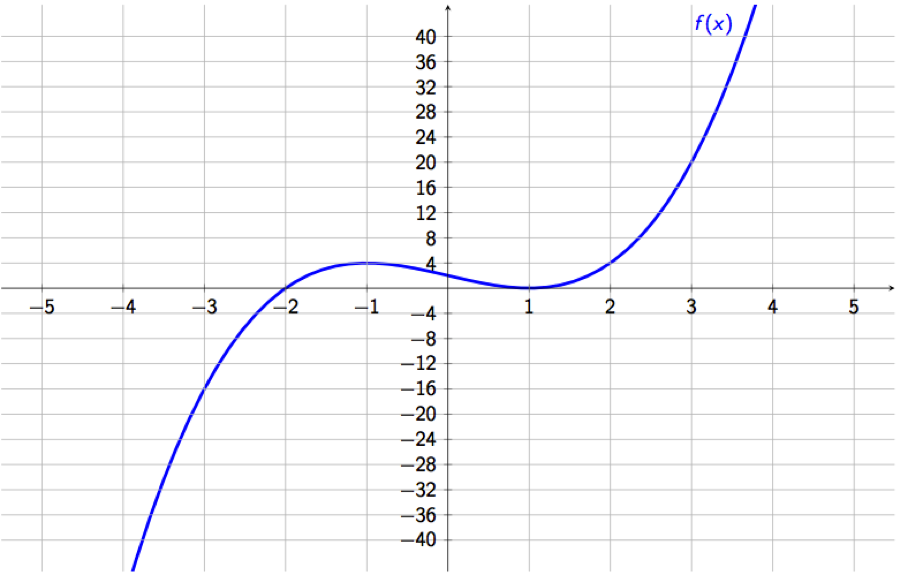
\includegraphics[scale=0.7]{Graphing1.png} \end{center}

  \begin{multipleChoice}
      \choice[correct]{Yes, I could find $f(2)$.}
      \choice[correct]{Yes, but I would need to review some resources first.}
      \choice[correct]{No, I would need to learn/relearn how to do this.}
      \choice[correct]{I don't know.}
      \choice[correct]{I don't want to answer this question right now.}
  \end{multipleChoice}
  
\end{question}

\begin{question} 
    Could you find the solutions to $f(x) = 0$ using the graph below?
    
\begin{center} 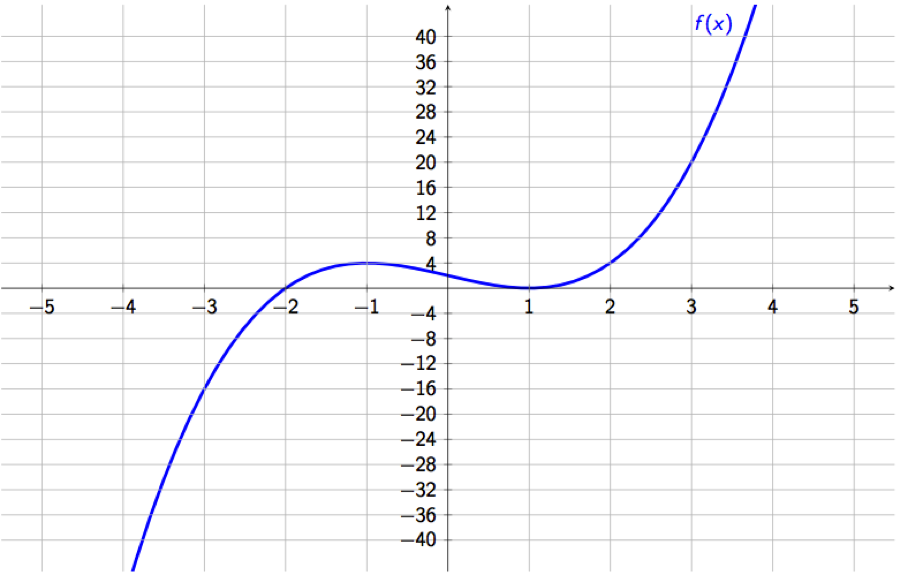
\includegraphics[scale=0.7]{Graphing1.png} \end{center}
  \begin{multipleChoice}
      \choice[correct]{Yes, I could find solutions to $f(x) = 0$.}
      \choice[correct]{Yes, but I would need to review some resources first.}
      \choice[correct]{No, I would need to learn/relearn how to do this.}
      \choice[correct]{I don't know.}
      \choice[correct]{I don't want to answer this question right now.}
  \end{multipleChoice}
  
\end{question}

\begin{question} 
    Given the function $f(x) = -3x + 2$, could you identify all interpretations of what `$f(2)$' represents?
    
  \begin{multipleChoice}
      \choice[correct]{Yes, I could identify all interpretations of $f(2)$.}
      \choice[correct]{I could identify some interpretations, but I would need to use other resources \\ to determine if the other interpretations were valid or not.}
      \choice[correct]{I know only one interpretation of what  `$f(2)$' represents, and I would need \\ to use resources to find any other interpretations of  `$f(2)$'.}
      \choice[correct]{No, I don't know any interpretations of `$f(2)$', and would need to learn/relearn what these are.
}
      \choice[correct]{I don't know.}
      \choice[correct]{I don't want to answer this question right now.}
  \end{multipleChoice}
\end{question}

\begin{question} 
    Given the function $f(x) = -3x + 2$, could you find all interpretations of the solution to $f(x) = 2$?
    
  \begin{multipleChoice}
      \choice[correct]{Yes, I could identify all interpretations of the solution to $f(x)=2$.}
      \choice[correct]{I could identify some interpretations, but I would need to refer to resources \\ to determine whether other interpretations were valid or not}
      \choice[correct]{I know only one interpretation of what the solution to  `$f(x)=2$' represents, and I would need \\ to use resources to find any other interpretations of what the solution to '$f(x)=2$' means.}
      \choice[correct]{No, I would need to learn/relearn how to do this.}
      \choice[correct]{I don't know.}
      \choice[correct]{I don't want to analyze this task right now.}
  \end{multipleChoice}
\end{question}

%Content Questions

\begin{problem} 

\begin{problem}
    Given the graph of the function $f(x)$ below, what is the value of $f(2)$?
    
    \begin{hint}
    HINT!
    \end{hint}
    
\begin{center} 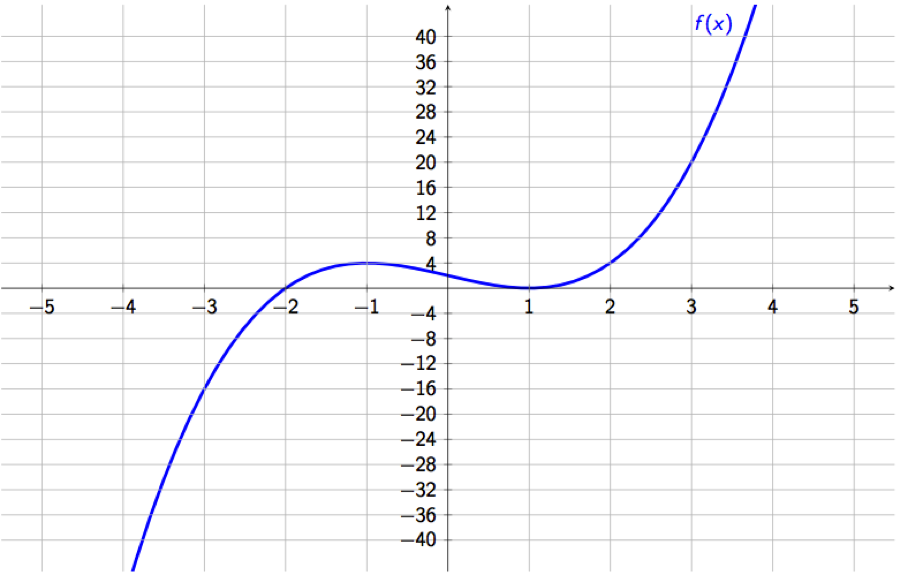
\includegraphics[scale=0.7]{Graphing1.png} \end{center}

  \begin{multipleChoice}
      \choice{$0$}
      \choice{$1$}
      \choice{$2$}
      \choice[correct]{$4$}
      \choice{$-1$ and $2$}
      \choice{$2.75$, $0.33$, and $1.5$}
      
      \begin{feedback}[attempt]
      Feedback.
      \end{feedback}
      
  \end{multipleChoice}
  
\end{problem}

\begin{question}
  
  If you didn't, why didn't you answer the above question?
  
  \begin{multipleChoice}
      \choice[correct]{I don't know the answer to this question yet.}
      \choice[correct]{I don't want to answer this question right now.}
      \choice[correct]{I have already answered this question correctly.}  
      
      \begin{feedback}[attempt]
      Feedback.
      \end{feedback}
  \end{multipleChoice}
  
\end{question}
  
\end{problem}

\begin{problem}

\begin{problem} 
    Given the graph of the function $f(x)$ below, what are the solutions to $f(x) = 0$?
    
    \begin{hint}
    Resource.
    \end{hint}
       
\begin{center} 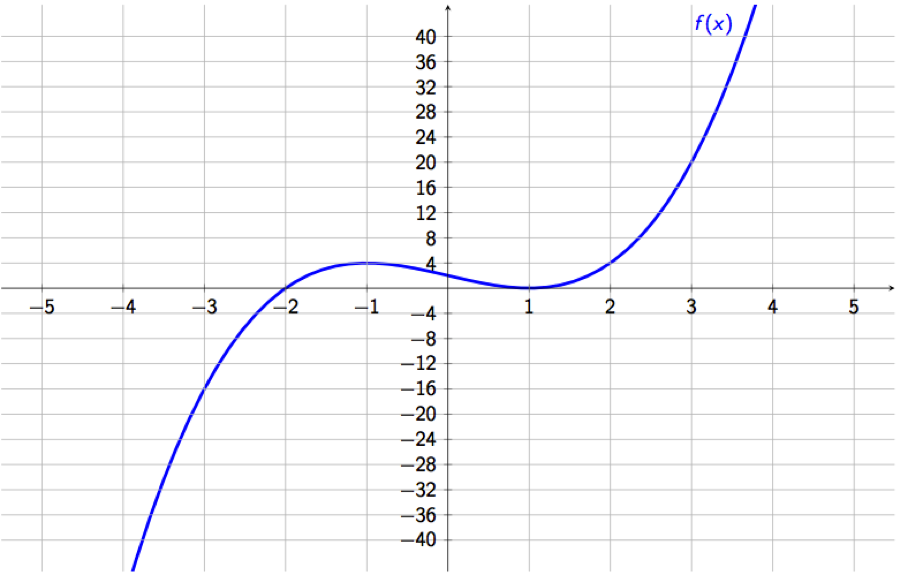
\includegraphics[scale=0.7]{Graphing1.png} \end{center}
    
  \begin{multipleChoice}
      \choice{$0$}
      \choice{$-2$}
      \choice{$1$}
      \choice{$2$}
      \choice{$-2$ and $0$}
      \choice[correct]{$-2$ and $1$}
      
     \begin{feedback}[attempt]
      Feedback.
      \end{feedback}
     
  \end{multipleChoice}
  
\end{problem}
\begin{question}
 
  
If you didn't, why didn't you answer the above question?
  
  \begin{multipleChoice}
      \choice[correct]{I don't know the answer to this question yet.}
      \choice[correct]{I don't want to answer this question right now.}
      \choice[correct]{I have already answered this question correctly.}
      
      \begin{feedback}[attempt]
      Feedback.
      \end{feedback}
      
  \end{multipleChoice}
  
\end{question}
  
\end{problem}

\begin{problem}

\begin{problem} 
    Consider the function $g(x) = -3x + 2$, what does $g(2)$ represent? \\ (Mark all that apply)
    
    \begin{hint}
    Resource.
    \end{hint}
    
  \begin{selectAll}
      \choice{A. The function gets multiplied by 2.}
      \choice[correct]{B. The function evaluated at 2.}
      \choice[correct]{C. The $y$-value on the graph of the function with $x$-coordinate 2.}
      \choice{D. The $x$-value on the graph of the function with $y$-coordinate 2.}
      \choice[correct]{E. The height of the graph of the function at $x=2$.}
      \choice[correct]{F. The distance between the graph of the function at $x=2$ and the $x$-axis.}
      \choice{G. The distance between the graph of the function at $y=2$ and the $y$-axis.}
      \choice{H. The slope of the graph of the function at $x=2$.}
      \choice[correct]{I. $-3(2) + 2$.}
      
      \begin{feedback}[attempt]
      Feedback.
      \end{feedback}
      
  \end{selectAll}
  
\end{problem}
\begin{question}
  
  If you didn't, why didn't you answer the above question?
  
  \begin{multipleChoice}
      \choice[correct]{I don't know the answer to this question yet.}
      \choice[correct]{I don't want to answer this question right now.}
      \choice[correct]{I have already answered this question correctly.}
      
      \begin{feedback}[attempt]
      Feedback.
      \end{feedback}
      
  \end{multipleChoice}
  
\end{question}

\end{problem}

\begin{problem}

\begin{problem} 
    Consider the function $g(x) = -3x + 2$, what does the solution of \\ $g(x)=2$ represent? (Mark all that apply)
    
    \begin{hint}
    Resource.
    \end{hint}
    
  \begin{selectAll}
      \choice{A. The function gets multiplied by 2.}
      \choice{B. The function evaluated at 2.}
      \choice{C. The $y$-value on the graph of the function with $x$-coordinate 2.}
      \choice[correct]{D. The $x$-value on the graph of the function with $y$-coordinate 2.}
      \choice{E. The height of the graph of the function at $x=2$.}
      \choice{F. The distance between the graph of the function at $x=2$ and the $x$-axis.}
      \choice[correct]{G. The distance between the graph of the function at $y=2$ and the $y$-axis.}
      \choice{H. The slope of the graph of the function at $x=2$.}
      \choice{I. $-3(2) + 2$.}
      
      \begin{feedback}[attempt]
      Feedback.
      \end{feedback}
      
  \end{selectAll}
  
\end{problem}
\begin{question}
  
    If you didn't, why didn't you answer the above question?
  
  \begin{multipleChoice}
      \choice[correct]{I don't know the answer to this question yet.}
      \choice[correct]{I don't want to answer this question right now.}
      \choice[correct]{I have already answered this question correctly.}
      
      \begin{feedback}[attempt]
      Feedback.
      \end{feedback}
      
  \end{multipleChoice}
  
\end{question}
  
\end{problem}

%Self-Control Questions

\begin{center} \textbf{Strategy Reflection}\end{center}

\begin{question}

Below are statements about strategies that you may or may not have used while completing the above questions.  Mark true or false to indicate whether each statement describes how you took this pre-quiz. 

\begin{question}

A. I answered the questions in order, assuming that the easier ones would come first.

    \begin{multipleChoice}
        \choice[correct]{True}
        \choice[correct]{False}
    \end{multipleChoice}
    
\end{question}
\begin{question}
    
    B. I answered the questions that I knew how to do first.

    \begin{multipleChoice}
        \choice[correct]{True}
        \choice[correct]{False}
    \end{multipleChoice}
    
\end{question}
\begin{question}
    
    C. I read through all of the questions first before answering any.

    \begin{multipleChoice}
        \choice[correct]{True}
        \choice[correct]{False}
    \end{multipleChoice}
    
\end{question}
\begin{question}
    
    D. After reading a question, I worked backwards and used process of elimination to narrow down my options by checking if the answers were correct.

    \begin{multipleChoice}
        \choice[correct]{True}
        \choice[correct]{False}
    \end{multipleChoice}
    
\end{question}
\begin{question}    
    
    E. I used online resources to find the solutions.

    \begin{multipleChoice}
        \choice[correct]{True}
        \choice[correct]{False}
    \end{multipleChoice}
    
\end{question}
\begin{question}    
    
    F. I used online resources to remind me how to answer the questions, but then solved them myself.

    \begin{multipleChoice}
        \choice[correct]{True}
        \choice[correct]{False}
    \end{multipleChoice}
    
\end{question}
\begin{question}    
    
    G. I used strategies when completing this pre-quiz, but I don't remember the names of the strategies.

    \begin{multipleChoice}
        \choice[correct]{True}
        \choice[correct]{False}
    \end{multipleChoice}
    
\end{question}
\begin{question}    
    
    H. I used other strategies that are not listed here.

    \begin{multipleChoice}
        \choice[correct]{True}
        \choice[correct]{False}
    \end{multipleChoice}
    
\end{question}
\begin{question}    
    
    I. I did not use any strategies when completing this pre-quiz.

    \begin{multipleChoice}
        \choice[correct]{True}
        \choice[correct]{False}
    \end{multipleChoice}

\end{question}
\end{question}


\begin{question}
    Please list any additional strategies that you used when taking this pre-quiz. If you didn't use any additional strategies, just type `NA.`
   \begin{freeResponse}
   \end{freeResponse}
\end{question}



%%% \begin{xarmaBoost}
%%   Write down at least \textbf{five} questions for this lecture. After
%%   you have your questions, label them as ``Level 1,'' ``Level 2,'' or
%%   ``Level 3'' where:
%% \begin{description}
%% \item[Level 1] Means you know the answer, or know exactly how to do
%%   this problem.
%% \item[Level 2] Means you think you know how to do the problem.
%% \item[Level 3] Means you have no idea how to do the problem.
%% \end{description}
%% \begin{freeResponse}
%% \end{freeResponse}
%% \end{xarmaBoost}



\end{document}
